\documentclass[%
  handout,
  aspectratio=1610,
  10pt,
  onlytextwidth, % requires Beamer v3.65 or newer
]{beamer}

\usepackage[T1]{fontenc}
\usepackage[english]{babel}
\usepackage[figurename=Fig.]{caption}
\usepackage{graphicx}
\usepackage{amsmath}
\usepackage{lipsum}
\usepackage{tikz}
\usepackage{scrextend}
\usepackage{ragged2e}
\usepackage[  
  style=numeric,
  sorting=nyt,
  sortcites,
  backend=biber   % use modern bibliography backend
]{biblatex}

% alternative: FiraSans
\usepackage[scaled]{helvet}

\usetheme{Wismar}

% presentation title (short version in brackets)
\title[Lorem Ipsum]{Lorem Ipsum}

% subtitle (optional)
\subtitle{Dolor sit amet}

% date (and place)
\date{Utopia, 1984}

% author / presenter (short version in brackets)
\author[J. Doe]{Jane Doe\\\href{mailto:j.doe@mail.com}{j.doe@mail.com}}

\institute{Faculty of Pseodoscience}

% project or faculty homepage (this is a custom macro from the Wismar theme)
\homepage{\url{https://theuselessweb.com}}

\usecolortheme{FIW}
% \usecolortheme{FWW}
% \usecolortheme{FG}

% disable navigation symbols globally
% \beamertemplatenavigationsymbolsempty

\addbibresource{quellen.bib}

\begin{document}

% title page
\maketitle

\begin{frame}
  \begin{abstract}
    \justifying
    \lipsum[1]
  \end{abstract}
\end{frame}

\begin{frame}{Outline}
  \tableofcontents
\end{frame}

\section{Frame elements}

\begin{frame}{\secname}{Subtitle}
  \lipsum[2]
  \footnote{This is not a real language!}
\end{frame}

\begin{frame}{\secname}{Columns}
  \begin{columns}
    \begin{column}[t]{0.49\textwidth}
      \justifying
      \lipsum[3][1-5]
    \end{column}
    \quad
    \begin{column}[t]{0.49\textwidth}
      \justifying
      \lipsum[3][6-10]
    \end{column}
  \end{columns}
\end{frame}

\begin{frame}{\secname}{Lists}
  \begin{columns}
    \begin{column}{0.5\textwidth}
      \begin{itemize}
        \item<+->first item
        \item<+->second item
        \begin{itemize}
          \item<+->nested item
          \begin{itemize}
            \item<+->third level of nesting
          \end{itemize}
          \item<+->another one
        \end{itemize}
        \item<+->\ldots
      \end{itemize}
    \end{column}

    \begin{column}{0.5\textwidth}
      \begin{enumerate}
        \item<+->one
        \item<+->two
        \item<+->three
      \end{enumerate}
    \end{column}
  \end{columns}
\end{frame}

\begin{frame}{Descriptions}
  \begin{columns}
    \begin{column}{0.5\textwidth}
      aligned at description:
      \begin{description}
        \item[Apple] sample text
        \item[Banana] sample text
        \item[Clementine] sample text
      \end{description}
    \end{column}

    \begin{column}{0.5\textwidth}
      aligned at label (requires package \texttt{scrextend}):
      \begin{labeling}{longest word}
        \item[long word] sample text
        \item[longer word] sample text
        \item[longest word] sample text
      \end{labeling}
    \end{column}
  \end{columns}
\end{frame}

\begin{frame}{Blocks}
  \begin{block}{Title}
    Block with title
  \end{block}

  \begin{block}{}
    Block without title
  \end{block}

  \begin{exampleblock}{Title}
    Example block with title
  \end{exampleblock}

  \begin{exampleblock}{}
    Example block without title
  \end{exampleblock}

  \begin{alertblock}{Title}
    Alert block with title
  \end{alertblock}

  \begin{alertblock}{}
    Alert block without title
  \end{alertblock}
\end{frame}

\begin{frame}{Theorems and Proofs}
  \begin{theorem}
    If $a$ and $b$ are the lengths of the sides adjacent to the right angle, the cathetus, and $c$ is the length of the side opposite the right angle, the hypotenuse (cf. figure \ref{fig:pythagoras}).
    \begin{equation*}\label{eq:pythagoras}
      c = \sqrt{a^2 + b^2}
    \end{equation*}
  \end{theorem}

  \begin{columns}
    \begin{column}{0.5\textwidth}
      \begin{figure}
        \centering{%
          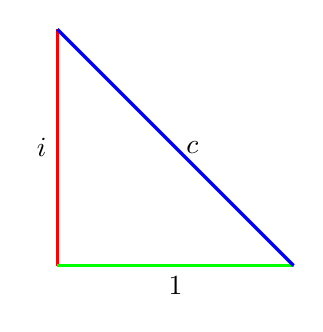
\begin{tikzpicture}
            \draw[red, very thick] (0,3) -- (0,0) node[left, pos=0.5, black] {$i$};
            \draw[green, very thick] (0,0) -- (3,0) node[below, pos=0.5, black] {$1$};
            \draw[blue, very thick] (0,3) -- (3,0) node[right, pos=0.5, black] {$c$};
          \end{tikzpicture}
          \caption{Visualization of Pythagoras' theorem}
          \label{fig:pythagoras}
        }
      \end{figure}
    \end{column}
    \begin{column}{0.5\textwidth}
      \begin{proof}
        \begin{displaymath}
          \begin{aligned}
            c & = \sqrt{i^2+1^2} \\
              & = \sqrt{-1 + 1}  \\
              & = \sqrt{0}       \\
              & = 0
          \end{aligned}
        \end{displaymath}
      \end{proof}
    \end{column}
  \end{columns}
\end{frame}

\section{Bounding box}

% testing the bounding box dimensions
\begin{frame}
  \centering
  
\begin{tikzpicture}[scale=0.99]
    \draw[red] (0,0) rectangle (\textwidth,\textheight);
    \draw[blue] (0,\textheight) -- (\textwidth,0)
    (0,0) -- (\textwidth, \textheight);
  \end{tikzpicture}
\end{frame}

\begin{frame}{Literaturverzeichnis}
  \printbibliography
\end{frame}

\finalpage{Thank you for your attention!}

\end{document}
